
    \documentclass{article}
    \usepackage[a4paper, left=2cm, right=2cm, top=1cm, bottom=2cm]{geometry}
    \usepackage{amsmath}
    \usepackage{graphicx}
    \begin{document}

    \begin{figure}[h!]
        \centering
        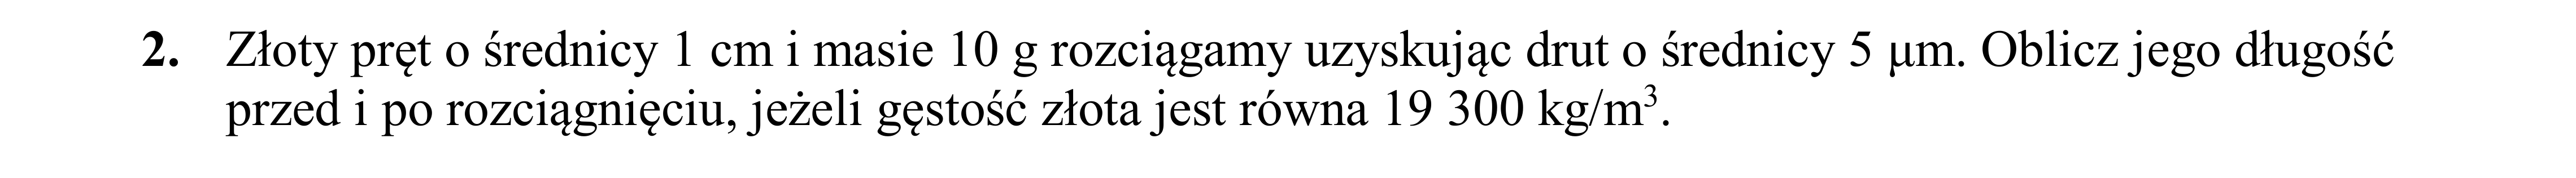
\includegraphics[width=1\textwidth]{Solutions/Zestaw 01/desc_02.png}
    \end{figure}

    \begin{quote}
    Aby obliczyć długość rozciągniętego drutu, można zastosować zasady związane z objętością i gęstością.

1. **Dane z zadania:**
   - Średnica pręta: \(d_1 = 1 \, \text{cm} = 0.01 \, \text{m}\)
   - Masa pręta: \(m = 10 \, \text{g} = 0.01 \, \text{kg}\)
   - Gęstość złota: \(\rho = 19300 \, \text{kg/m}^3\)
   - Średnica drutu: \(d_2 = 5 \, \mu m = 5 \times 10^{-6} \, \text{m}\)

2. **Oblicz objętość pręta złotego:**
   \[
   V = \frac{m}{\rho} = \frac{0.01 \, \text{kg}}{19300 \, \text{kg/m}^3} \approx 5.18 \times 10^{-7} \, \text{m}^3
   \]

3. **Oblicz objętość drutu:**
   ObjVolume of a cylinder (drut) is given by:
   \[
   V = \pi r^2 h
   \]
   gdzie \(r = \frac{d_2}{2}\) oraz \(h\) to długość drutu, którą chcemy znaleźć.

   \[
   r_2 = \frac{5 \times 10^{-6}}{2} = 2.5 \times 10^{-6} \, \text{m}
   \]

4. **Równanie związane z objętościami:**
   Objętość pręta (która jest objętością drutu po rozciągnięciu) jest taka sama, więc:
   \[
   V_1 = V_2 \implies \frac{m}{\rho} = \pi (2.5 \times 10^{-6})^2 h
   \]

5. **Oblicz długość drutu \(h\):**
   \[
   5.18 \times 10^{-7} = \pi (2.5 \times 10^{-6})^2 h
   \]

   \[
   h = \frac{5.18 \times 10^{-7}}{\pi (2.5 \times 10^{-6})^2}
   \]

   \[
   h = \frac{5.18 \times 10^{-7}}{\pi \times 6.25 \times 10^{-12}} \approx \frac{5.18 \times 10^{-7}}{1.9635 \times 10^{-11}} \approx 26.3 \, \text{m}
   \]

**Ostateczny wynik:** Długość drutu po rozciągnięciu wynosi około **26.3 m**.
    \end{quote}
    \end{document}
    